\documentclass{hagaki-doc}

\title{Hagaki クラス}
\author{HiroSpark}
\date{v0.1.0}

\begin{document}

\maketitle

\section{概要}

\code{Hagaki} クラスはハガキの宛名印刷を簡単に行うためのドキュメントクラスです。
Lua\LaTeX{} が必要です。

\section{インストール}

リポジトリをクローンし、\file{build.lua}のあるディレクトリで、

\begin{lstlisting}
$ l3build install
\end{lstlisting}

を実行してください。
\pkg{l3build}によって、TDSに準拠した形で、\code{TEXMF}ツリーに
\file{hagaki.cls}がインストールされます。
アンインストールするには、同じディレクトリで、

\begin{lstlisting}
$ l3build uninstall
\end{lstlisting}

を実行します。
詳細は\pkg{l3build}のドキュメントを見てください。

\section{使用法}

予定にはありませんが、現在も開発中なため、将来のリリースで変更される可能性があります。
\cmd{sender}は差出人の情報を、\cmd{recipient}は宛先の情報を指定します。
\cmd{recipient}は宛先の情報の指定とともに、宛名面の作成も行います。

どちらも|keyval|リストで郵便番号・住所・名前を指定します。
受け取る値の詳細は以下のようになっています。

\begin{tabularx}{\linewidth}{llX}
  \toprule
  \code{key} & 指定する値 & 注意 \\
  \midrule
  \code{postal\_code} & 郵便番号 & \code{-} が必要です。\\
  \code{name} & 名前 & 半角スペースで名字と名前を区切ってください。\\
  \code{address} & 住所 &
  組版の関係で、英数字は「\rotatebox[origin=c]{270}{1}」のようになってしまいます。
  それを避けたい場合は、数字を和文文字にするか、\pkg{lltjext} の
  \cmd{rensuji{}} を使ってください。\\
  \bottomrule
\end{tabularx}

例えば、以下のソースを処理すると、次のような宛名面が作成されます。

\begin{lstlisting}
\documentclass{hagaki}
\sender{
  postal_code = 103-0027,
  name        = 日本 太郎,
  address     = 東京都中央区日本橋1-3-11
}
\begin{document}
\recipient{
  postal_code = 542-0071,
  name        = 戎 太郎,
  address     = 大阪府大阪市中央区道頓堀1丁目
}
\end{document}
\end{lstlisting}

\fbox{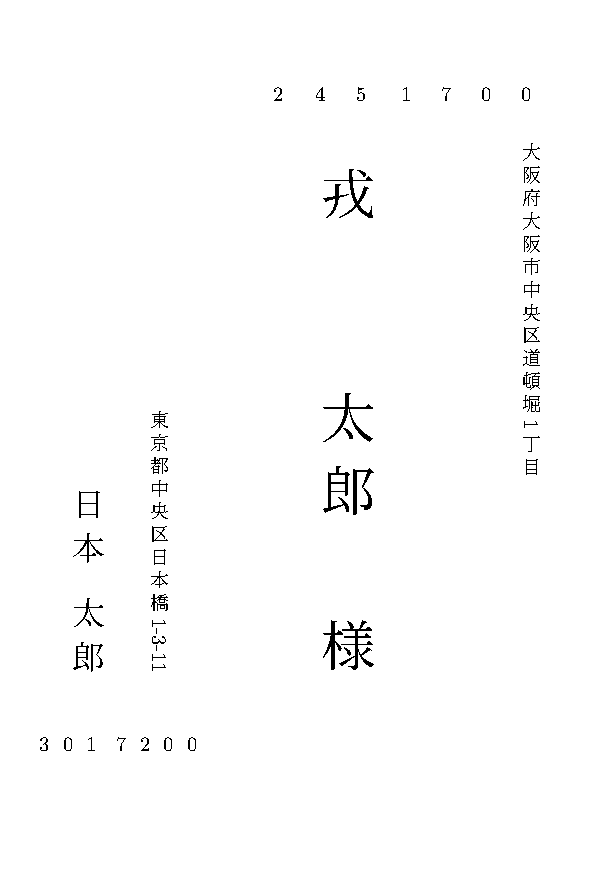
\includegraphics[width=.5\linewidth]{example.pdf}}

\end{document}